\section{Convolution}
This section introduces the convolution from a more mathematical perspective and then gives some less traditional applications of a more generalized version.

\subsection{Definition}
Conceptually, the convolution operation gives the overlap between two functions as a function of the offset between the functions.

Mathematically, convolution is defined by an integral:

\[
    (f * g)(t) = \int^{\infty}_{-\infty}{f(\tau)g(t-\tau) d\tau}
\]

Its discrete counterpart is:

\[
    (f * g)(n) = \sum^{\infty}_{i=-\infty}{f(i)g(n-i)}
\]

\begin{figure}
    \centering
    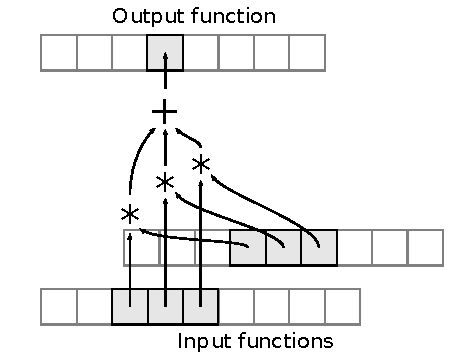
\includegraphics{img/VisualConvolution}
    \caption{
        Convolution performed on discrete functions.
        Each box represent an output value of the function.
    }
    \label{fig:VisualConvolution}
\end{figure}

This is visualized in figure \ref{fig:VisualConvolution} where we have focused on only 3 of the values in the input functions. Notice how the corresponding values from the input functions are multiplied together before the products are summed.

This can also be extended to multiple dimensions by summing across the additional dimensions.
For the discrete case, this gives
\[
    (f * g)(n, m) = \sum^{\infty}_{i=-\infty}\sum^{\infty}_{j=-\infty}{f(i, j)g(n-i, m-j)}
\]

\subsection{Application in Image Processing}
As mentioned in the introduction, convolution can be used in image processing to apply various filters to an image.

A monochrome image can be thought of as a 2D matrix with a width $W$ and height $H$.
Let $I(x, y)$ be a function for accessing a specific value in the image matrix.
Let $K(x, y)$ be a function for accessing a specific value in a special matrix called the \textit{kernel},
or $0$ if $x$ or $y$ is out of bounds for the matrix.

The convolution of the image and the kernel is then given by
\[
    C(x, y) = \sum^{H}_{h=0} \sum^{W}_{w=0}{I(w, h)K(w - x, h -y)}
\]
where $C(x, y)$ is the output image.

For a coloured image, each channel is processed separately.

Depending on the kernel matrix, various effects like blurring or sharpening may be applied to the image with convolution.
A small selection of possible kernel matrices and the results the produce can be found in table \ref{tab:KernelMatrices}.

\begin{table}
    \begin{tabular}{ccm{3cm}}
    Description & Matrix & Result \\
    \hline
    Blur & $
            \begin{bmatrix}
            1/9 & 1/9 & 1/9 \\
            1/9 & 1/9 & 1/9 \\
            1/9 & 1/9 & 1/9
            \end{bmatrix}
        $ & 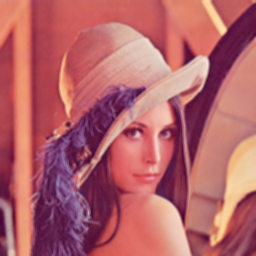
\includegraphics[width=3cm]{img/LenaBlurred} \\
    Edge-detect & $
            \begin{bmatrix}
            -1 & -1 & -1 \\
            -1 & 8 & -1 \\
            -1 & -1 & -1
            \end{bmatrix}
        $ & 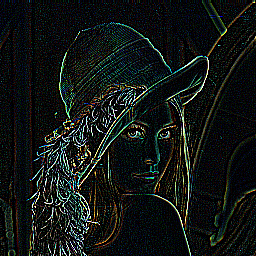
\includegraphics[width=3cm]{img/LenaEdge} \\
    Emboss & $
            \begin{bmatrix}
            -2 & -1 & 0 \\
            -1 & 1 & 1 \\
            0 & 1 & 2
            \end{bmatrix}
        $ & 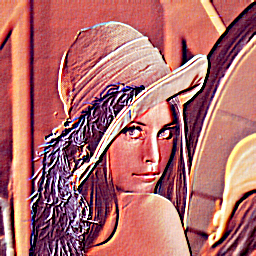
\includegraphics[width=3cm]{img/LenaEmbossed}
    \end{tabular}
    \caption{Some kernels used in image processing}
    \label{fig:KernelMatrices}
\end{table}

As the matrices in table \ref{tab:KernelMatrices} are good examples of, the kernel matrices used for image processing is usually small compared to the images, and often of a constant size.
This means each output pixel is a function of the same pixel in the original image and its neighbourhood.

\subsection{Generalized convolution}
Convolution can be separated into to phases; first we have the multiplication before a summation follows.
In our image processing application, the multiplication phase simply maps a set of input values to a set of output values.
These values are then reduced into one value by summation.

To generalize convolution, we can replace the map and reduce operations.
In our general case, a convolution operation is therefore fully defined by two input matrices and two operations.

In the realm of image processing, this paves the way for new filters, such as the median, minimum and maximum filters.
These filters are commonly used to remove noise in images and consists of a convolution kernel matrix filled with 1s (the multiplicative identity), the multiplication operation for the map stage and the minimum, maximum or mean operations respectively for the reduce operations.
The resulting images created by applying the effect to our test image can be seen in table \ref{tab:GeneralizedKernelMatrices}.

\begin{table}

    \begin{tabular}{lm{3cm}}
        Reduce operation & Result \\
        \hline
        Minimum & 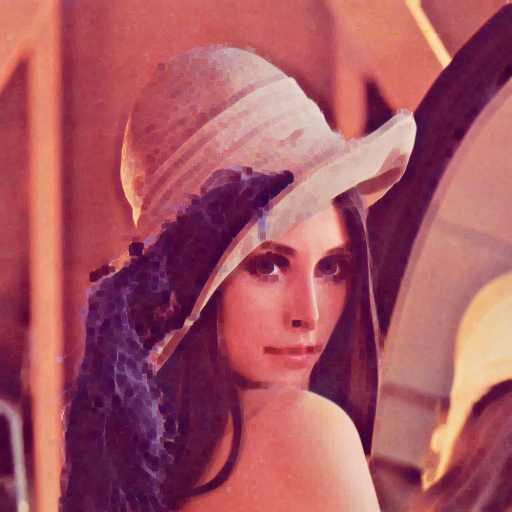
\includegraphics[width=3cm]{img/LenaMin} \\
        Maximum & 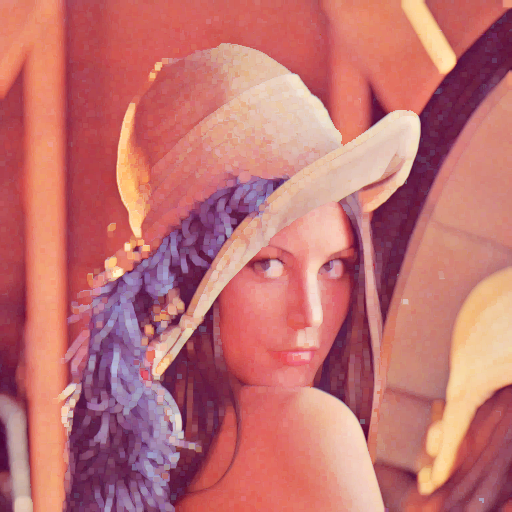
\includegraphics[width=3cm]{img/LenaMax} \\
        Median & 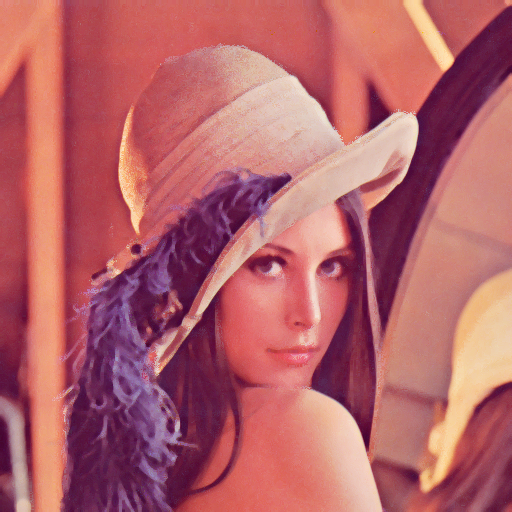
\includegraphics[width=3cm]{img/LenaMedian}
    \end{tabular}

    \caption{Some image processing filters using a generalized form of convolution}
    \label{tab:GeneralizedKernelMatrices}

\end{table}

Generalized convolution can also be used in other areas, such as to calculate the next iteration of cellular automatons. This requires a more advanced reduce operation.

\section{TODO: Implementing convolution}
Comment from Yaman on this section:
\begin{quotation}
the section heading "Implementing convolution" does not match the section content. what is the purpose of this section? is it background? is it meant to describe your own design decisions for the solution?

yes you can assume, bandwidth is a known constraint when working on data-intensive stuff.

but remember there are (generally speaking) two kinds of bandwidth in computing: "off-chip" and "on-chip". off-chip storage is large and low bandwidth, on-chip storage is small and high bandwidth. 

this is why we try to exploit "data reuse" as much as possible; keep the reused bits on-chip so we can access them again and again with high bandwidth.
\end{quotation}


On modern computers the memory bandwidth will usually be the bottleneck of any operation involving large amounts of data, such as an image. TODO reference (or is it considered common knowledge?)
The essence of implementing efficient convolution is therefore removing redundant data movement.
Whenever we move a pixel into working memory we ideally want to perform a map operation for every neighbourhood it is part of.
If a pixel is ejected from memory it will have to be retrieved again until all convolutions it is part of has been calculated.
Ideally we would have enough memory to store an entire image and work on all parts simultaneously. While this can certainly be done, if we want speed we have to sacrifice memory size.
The challenge is therefore to use as little memory as possible balanced with reducing redundant loads.\\

